% (c) GreenSocs Ltd
% author: Christian Schroeder <schroeder@eis.cs.tu-bs.de>

%%%%%%%%%%%%%%%%%%%%%%%%%%%%%%%%%%%%%%%%%%%
%%%%%%%%%%%%%%%%%%%%%%%%%%%%%%%%%%%%%%%%%%%
\chapter{General Project Handling}
\label{sec:GeneralProjectHandling}

This chapter is a short introduction how to prepare your project for PCIe.


%%%%%%%%%%%%%%%%%%%%%%%%%%%%%%%%%%%%%%%%%%%
\section{Global Project Settings}

For your global project settings we recommend to use a global setting file (e.g. \Datei{globals.h}) which is included by each header file before any other includes (expect systemc.h).

\ZwischenUberschrift{Debug Output}

In the global setting file you can switch on the PCIe terminal outputs by defining
\begin{lstlisting}
#define PCIeDEBUG_ON
\end{lstlisting}

To enable other GreenBus outputs use 
\begin{lstlisting}
#define VERBOSE
\end{lstlisting}


\ZwischenUberschrift{Additional PCIe Checks}

The PCIe implementation is prepared to check additional rules apart from the obligatory ones defined in the PCIe specification. To enable these additional checks, use
\begin{lstlisting}
#define CHECK_RULES_ENABLE
\end{lstlisting}
\Achtung{Note that these checks need some more run time. Disable these checks for large simulations where you already know that no failures occur.}

\ZwischenUberschrift{Static / Dynamic Casts}

The PCIe Transaction derivation tree can be compiled such that dynamic casts are needed (slower, old, depricated version) or the model can be compiled allowing static casts (faster, new version). The GreenBus default is the dynamic casts version due to compatibility reasons. Whenever possible \emph{use the static casts version} in PCIe projects by setting the define in the \Datei{globals.h}:
\begin{lstlisting}
#define USE_STATIC_CASTS
\end{lstlisting}

This User's Guide takes most focus on the static casts version. If nothing else is mentioned the descriptions are related to the static casts version,

\Note{Implementation Note}{Static / Dynamic Casts}{In principle a PCIe dynamic casts version topology should be able to work together in parallel with a generic topology using (real) \lstinline|GenericTransaction|s. But for code and usage clearness the define USE\_PCIE\_TRANSACTION has to be set in \mbox{\Datei{globals.h}.} Then the generic transaction, phase and access classes are typedefed to PCIe classes which may be used in a generic or a PCIe manner.}

\Achtung{Instead of defining the static or dynamic casts usage in the \Datei{globals.h} the chose can be done with the make switch \Eingabe{make STATIC=yes}. For more details see \Datei{greenbus/examples/README}.}


%%%%%%%%%%%%%%%%%%%%%%%%%%%%%%%%%%%%%%%%%%%
\section{Include PCIe.h}
\label{sec:IncludePCIe}

In \emph{each header} file of the PCIe project first include the user specific \Datei{globals.h} and afterwards \mbox{\Datei{PCIe.h}:}
\begin{lstlisting}
#include "globals.h"
#include "greenbus/transport/PCIe/PCIe.h"
\end{lstlisting}

The second include defines the PCIe Transaction and access classes and (in the case of static casts) typedefs the generic types to PCIe.

Generic devices may include \Datei{greenbus/transport/GP/GP.h} instead of \Datei{PCIe.h} if some settings in \Datei{globals.h} are done, see section \ref{sec:GenericDevicesInPCIe}.

\Achtung{PCIe projects should be hard coded to use the PCIe Transactions by including \DateiNoImg{PCIe.h} -- see above. In the case of mixed projects with generic devices -- which include \DateiNoImg{GP.h} -- the user can enable the PCIe Transaction with a make switch instead of including an user defined \mbox{\DateiNoImg{globals.h}:} \Eingabe{make EXTENSION=PCIe}. Also see  \Datei{greenbus/examples/README} for more details.}


%%%%%%%%%%%%%%%%%%%%%%%%%%%%%%%%%%%%%%%%%%%
\section{Generic Devices in PCIe}
\label{sec:GenericDevicesInPCIe}

When combining generic and PCIe peripherals together within a PCIe project use the static casts version. In the generic peripherals' header files the user has to take care of using the PCIe Transaction definition either by global define or by make file switch (see section \ref{sec:IncludePCIe}).

All generic types are typedefed to PCIe types (e.g. \lstinline|GenericTransaction| = \mbox{\lstinline|PCIeTransaction|,} \lstinline|GenericMasterAccess| = \lstinline|PCIeMasterAccess|).

In the case the dynamic casts version is used together with generic ports, routers, devices etc, define the following defines in the \Datei{globals.h}:
\lstinline[language=TeX]|#define EXTENDED_TRANSACTION PCIe| (Uses PCIe transaction), \lstinline[language=TeX]|#define USE_PCIE_TRANSACTION| (Enables typedefs Generic = PCIe)



%%%%%%%%%%%%%%%%%%%%%%%%%%%%%%%%%%%%%%%%%%%
%%%%%%%%%%%%%%%%%%%%%%%%%%%%%%%%%%%%%%%%%%%
\chapter{PCIe specific Classes}
\label{sec:PCIeSpecificClasses}

This chapter leads through the process of creating a project with PCIe Devices, Switches, Root Complex etc. In the end there is a section \ref{sec:MixGenericAndPCIeDevices} about how to connect generic devices to PCIe and vice versa.

%%%%%%%%%%%%%%%%%%%%%%%%%%%%%%%%%%%%%%%%%%%
\section{Transactions and Accesses}

Figure \ref{fig:TransactionDerivationTree} shows the derivation tree for static casts PCIe Transactions and Accesses.

The PCIe types are typedefed to generic types:
\begin{lstlisting}
typedef PCIe::PCIeTransaction GenericTransaction;
typedef PCIe::PCIeSlaveAccess GenericSlaveAccess;
typedef PCIe::PCIeMasterAccess GenericMasterAccess;
typedef PCIe::PCIeRouterAccess GenericRouterAccess;
typedef PCIe::PCIePhase GenericPhase;
\end{lstlisting}


\begin{figure}[htbp]%[H]%[htbp]
	\centerline{
		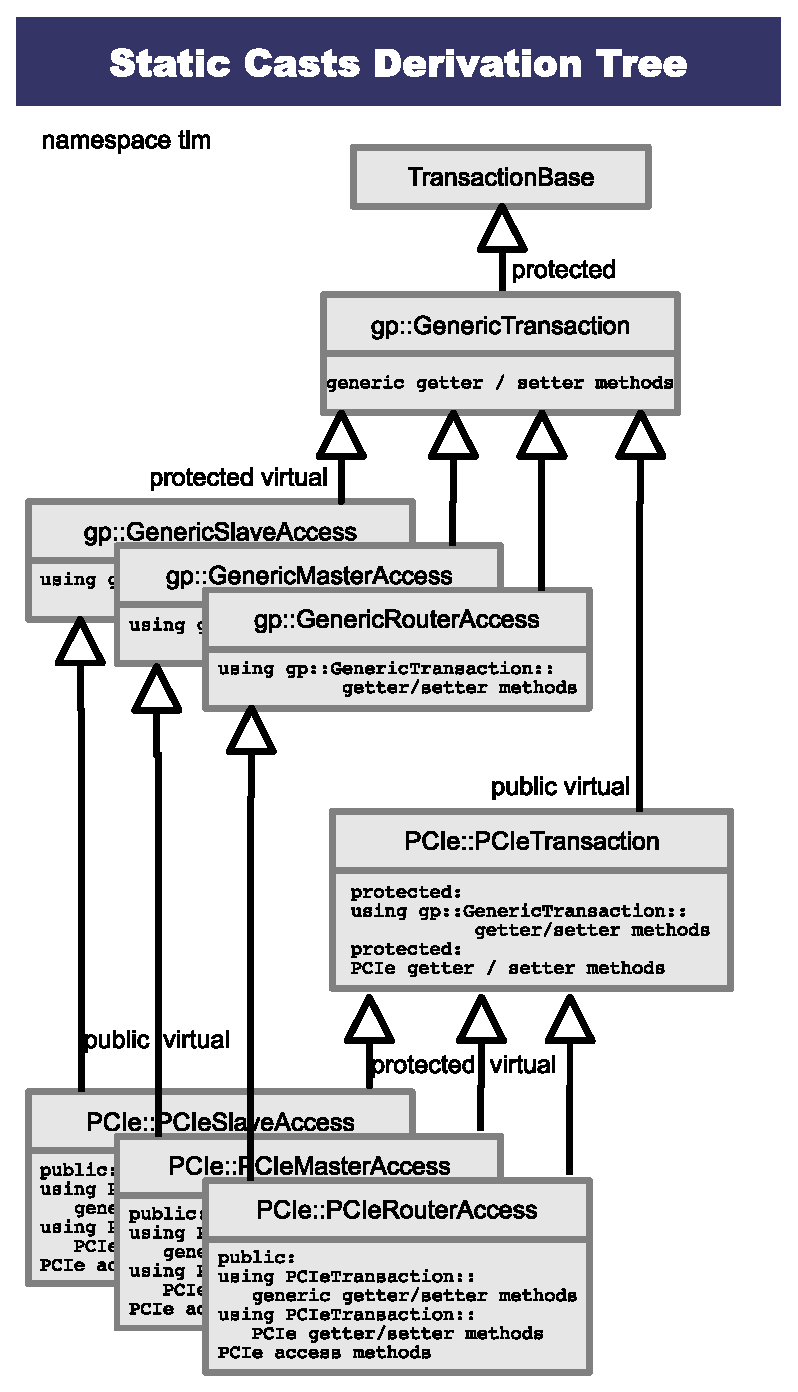
\includegraphics{figures/StaticTransactionDerivationTree.eps}} 
	\caption{Derivation tree Transactions, Accesses.}
	\label{fig:TransactionDerivationTree}
\end{figure}

The quark access methods in the PCIe Transaction class are protected to avoid the direct usage of the Transaction class. The user has to use the Access class which matches the actual usage type: When creating a transaction use the \lstinline|MasterAccess|, when processing a received transaction, use the \mbox{\lstinline|SlaveAccess|.} Smart pointers of these Access classes are typedefed to \mbox{\lstinline![Master|Slave]AccessHandle!.} Router Accesses are not covered in the document just as phases.

The user can use class methods to get Accesses out of a transaction:
\begin{lstlisting}
PCIeMasterAccess &getMasterAccess();
PCIeSlaveAccess &getSlaveAccess();
\end{lstlisting}

And the user can use global methods to get Access handles from Transactions and Atoms. (Atoms are not used in the PV implementation):
\begin{lstlisting}
GenericMasterAccessHandle _getMasterAccessHandle(/*Atom or Transaction*/)
GenericSlaveAccessHandle _getSlaveAccessHandle(/*Atom or Transaction*/)
\end{lstlisting}

How to use the access methods also see section \ref{sec:UsingThePCIeAPI}.

In a PCIe peripheral module the user instantiates the PCIe API (see section \ref{sec:UsingThePCIeAPI}). 

When creating a PCIe TLP the PCIe Master Access class provides convenience methods for all existing TLP types, e.g.:
\begin{lstlisting}
init_Memory_Read(/* address, data, data size, requester func. no. */);
init_Memory_Write(/* address, data, data size, requester func. no. */);
init_IO_Read(/* address, data, data size, requester function no. */);
init_IO_Write(/* address, data, data size, requester function no. */);
init_Configuration_Read(/* bus no., dev. no., func. no., ..., data, ...*/);
init_Configuration_Write(/* bus no., dev. no., func. no., ..., data, ...*/);
init_Message(/* message code, requester func. no. */);
\end{lstlisting}

When receiving and processing a PCIe TLP the PCIe Slave Access class provides convenience methods, e.g.:
\begin{lstlisting}
get_TLP_type();
get_addr();
init_Memory_Read_Completion(/* completion status, completer func. no. */);
// ...
set_Completion_Status(/* status */)
init_Unsupported_Request();
\end{lstlisting}

For the detailed and complete list of access methods look at the doxygen API reference.

%%%%%%%%%%%%%%%%%%%%%%%%%%%%%%%%%%%%%%%%%%%
\section{Using the PCIe API}
\label{sec:UsingThePCIeAPI}

The PCIe framework provides one API (\lstinline|PCIeAPI|) for PCIe peripherals independent from their main behavior as a master or slave since each PCIe device is a master \emph{and} a slave in (Green)Bus terms. Include \Datei{greenbus/api/PCIe/PCIeAPI.h} before using the API.

\Note{Implementation Note}{Bidirectional PCIe Ports}{Because each PCIe device is a bus master and a slave the PCIe API has one bidirectional port which acts as a master \emph{and} a slave. The bidirectional port \mbox{(\lstinline|PCIeBidirectionalPort|)} is a \lstinline|GenericInitiatorAPI| which is instantiated with the constructor parameter \mbox{\lstinline[language=TeX]|is_bidirectional=true|.}}

%%%%%
\subsection{Processing incoming TLPs}
The PCIe API creates a PCIe Configuration Space Header of type 0 (for PCIe device Functions) and handles the incoming Configuration Request TLPs automatically. The user module needs not to care about them. Details about Configuration Space see section \ref{sec:ConfigurationSpace}.

The API does some additional checks for incoming transactions. Some of the rule checks can be switched off by removing the define PRECHECK\_ENABLE in \Datei{greenbus/api/PCIe/PCIeAPI.h}. After these first checks the transaction is forwarded to the \lstinline|b_transact| method which has to be implemented by the user module. The user device has to implement the \lstinline|PCIe_recv_if| interface and give the this pointer to the API during its construction. Use the convenience methods of the Slave Access class to process the TLP in the switch statement. An example implementation of a sending and receiving PCIe device is presented in the example listing in figure \ref{fig:ListPCIeDevice}. See an example for a receiving device e.g. in \Datei{greenbus/examples/PCIe/platform/PCIeRecvinfoDevice.h}.

%%%%%
\subsection{Creating and sending TLPs}

The same PCIe API can be used for creating and sending TLPs.

Call the \mbox{\lstinline|create_transaction()|-}method on the API to get a Master Access Handle to the TLP which should be sent. Afterward call the convenience method(s) according to the TLP type you want to send. Call \mbox{\lstinline|myAPI.send(myMasterAccessHandle)|} on the API to send the TLP. In a final step process the completion of the TLP if there is one again using the convenience methods of the Access class.

See figure \ref{fig:ListPCIeDevice} for an example listing. Find an example for a sending device e.g. in \mbox{\Datei{greenbus/examples/PCIe/platform/PCIeSendDevice.h}.}

If a device should only send but not process received transactions the constructor of the API can be called with NULL instead of the this pointer. Then the API will internally process the transactions (e.g. handle Configuration Requests and manipulate the Configuration Space) but will not try to forward them to the user device implementation. If a transaction is received which needed user processing an sc\_warning will be reported.

\begin{figure}[H]%[htbp]
  \begin{lstlisting}
#include "my_globals.h"
#include "greenbus/transport/PCIe/PCIe.h"
#include "greenbus/api/PCIe/PCIeAPI.h"
using namespace tlm;
using namespace tlm::PCIe;

class MyPCIeDevice
 : public sc_module,
   public tlm::PCIe::PCIe_recv_if // for receiving ability {
public:
  PCIeAPI myAPI;

  SC_HAS_PROCESS(MyPCIeDevice);
  MyPCIeDevice(sc_module_name name)
   : sc_module(name),
     myAPI("PCIeAPI", this) // for sending and receiving
  {
    SC_THREAD(send_action); // for sending
  }
  
  /// Method for receiving ability
  virtual void b_transact(PCIeTransactionHandle th) {
    PCIeSlaveAccessHandle ah = _getSlaveAccessHandle(th);

    switch((unsigned int)th->get_TLP_type()) {
      case MemWrite:
      // ...
  }  }
  
  /// Thread for sending ability
  void PCIeSendDevice::main_action() {
    // dummy data
    std::vector<gs_uint8> *dat;
    dat = new std::vector<gs_uint8>(data_size);
    for (unsigned int i = 0; i < data_size; i++) dat->at(i) = i;

    // create transaction
    PCIeMasterAccessHandle ah;
    ah = mAPI.create_transaction();
    // fill transaction with data
    ah->init_IO_Write( addr, *dat, data_size );
    // send transaction
    mAPI.send_transaction(ah);

    // process Completion    
    if (ah->get_Completion_Status() == SuccessfulCompletion) {
      /* process data */
    } else { /* Completion not successfull */ }
    delete dat; dat = NULL;
} }
  \end{lstlisting}
  \caption{Example listing PCIe device.}
  \label{fig:ListPCIeDevice}
\end{figure}

%%%%%%%%%%%%%%%%%%%%%%%%%%%%%%%%%%%%%%%%%%%
\section{Configuration Space}
\label{sec:ConfigurationSpace}

TODO: The Configuration Space is not yet implemented. We are waiting for DRF.

%%%%%%%%%%%%%%%%%%%%%%%%%%%%%%%%%%%%%%%%%%%
\section{Addressing}
\label{sec:Addressing}

The PCIe framework supports the three address (routing) types of PCIe: address based, ID based and implicit routing.

The PCIe Transaction has two boolean variables which store the kind of used address type due to fast access (figure \ref{fig:RoutingTypes}):

\begin{figure}[H]
  \centerline{
  \begin{tabular}{|l||l|l|l|}
    \hline
     & \textsf{Address based Routing} & \textsf{ID based routing} & \textsf{Implicit routing} \\
    \hline
    \hline
    \textsf{mIsIDbasedRouting} &  false & \emph{true} & false \\
    \textsf{mIsImplicitRouting} &  false & false & \emph{true} \\
    \hline
  \end{tabular}
  }
  \caption{Routing types.}
  \label{fig:RoutingTypes}
\end{figure}

\ZwischenUberschrift{Address based routing}

The address based routing is divided into two independent address spaces: \emph{Memory address space} and \emph{I/O address space}. The routing information is transported in the quark \lstinline|mAddr| which is the default quark for addresses in GreenBus. GreenBus routing with MAddr matches address based routing. Other routing mechanisms cannot be mapped to MAddr field routing because all 64 bit are needed by address based routing.

\ZwischenUberschrift{ID based routing}

The PCIe ID based routing is mapped to the quarks \lstinline|mBusNo|, \lstinline|mDevNo|, \lstinline|mFuncNo| and \lstinline|mRegNo|. ID based routing is needed for Configuration Requests. The Requester ID is the ID of a TLP's sender. The user needs not to handle these addresses. Only the Root Complex implemenatation gets in contact with the IDs. Requester IDs are set automatically by the API.

\ZwischenUberschrift{Implicit routing}

Implicit routing is done with the quark \lstinline|mMessageType|.
The user needs not to handle implicit routing. The message creating convenience methods set the correct values.

\begin{figure}[H]
  \centerline{
  \begin{tabular}{|l|l|l|}
   \hline
   \textsf{RoutedToRootComplex}              &  000    &  Route to Root Complex    \\ 
   \hline
   \textsf{RoutedByAddress}                  &  001    &  Never used \\
    & & (mIsIDbasedRouting=mIsImplicitRouting=false)   \\ 
   \hline
   \textsf{RoutedByID}                       &  010    &  Route normally by ID \\
    & & (set mIsIDbasedRouting=true \\
    & & instead of mIsImplicitRouting!)   \\ 
   \hline
   \textsf{BroadcastFromRootComplex}         &  011    &  Broadcast from Root Complex to all devices   \\ 
   \hline
   \textsf{LocalTerminateAtReceiver}         &  100    &  Local - Not forwarded at the next switch   \\ 
   \hline
   \textsf{GatheredAndRoutedToRootComplex}    &  101    &  see PME\_TO\_Ack Message Code: \\
    & &  Collect Acks from Downstream Ports \\
    & & and send one to Upstream Port  \\ 
   \hline
\end{tabular}
  }
  \caption{Implicit routing types.}
  \label{fig:ImplicitRoutingTypes}
\end{figure}


%%%%%%%%%%%%%%%%%%%%%%%%%%%%%%%%%%%%%%%%%%%
\section{Switch}

The PCIe Switch class is named \lstinline|PCIeRouter| following the GreenBus terms. A Switch has an Upstream Port (\lstinline|upstream_port|) which has to be connected to another bidirectional PCIe port: a Downstream Port of another Switch or a Root Complex. The Downstream Port of a Switch is a multi port. The user can connect one or more bidirectional PCIe ports to this port: mainly that will be PCIe device's or other Switch's Upstream Ports. (The Downstream port is not needed to be connected to any port. It may left unbound.)

Generic devices may be connected to the Downstream Port according the rules in section \ref{sec:MixGenericAndPCIeDevices}.


%%%%%%%%%%%%%%%%%%%%%%%%%%%%%%%%%%%%%%%%%%%
\section{Root Complex}

The Root Complex is a device with an internal PCIe Switch. To help the user with implementing the Root Complex there is a class \lstinline|PCIeRootComplex| (see \Datei{greenbus/api/PCIe/PCIeRootComplex.h}). This derives from the \lstinline|PCIeRouter| class, accordingly the user is able to connect devices and switches to its Downstream Port. Do not connect the Upstream Port: it is bound internally to the \lstinline|down_to_router_port| which is another PCIeAPI port. That port is the connection from the software/CPU to PCIe and should be used by the user to implement the Root Complex functionality.

At minimum the user has to implement the method \lstinline|PCIeRootComplex::down_to_router_port_b_transact(PCIeTransactionHandle th)|. To be able to extend the Root Complex the user should derive from this class, e.g. \lstinline[language=TeX]|MyPCIeRootComplex : public PCIeRootComplex|. 
See \Verzeichnis{greenbus/examples/PCIe/platform} for an example.

\begin{itemize}
  \item The \lstinline|PCIeRootComplex| is a (derives from) \lstinline|PCIeRouter|.
  \item Use Downstream Port to connect the PCIe tree topology.
  \item Do not use the Upstream Port which is connected internally.
  \item Use the port \lstinline|down_to_router_port| to access the PCIe topology.
  \item Implement \lstinline|down_to_router_port_b_transact| to handle incoming TLPs from the PCIe topology.
  \item Derive from \lstinline|PCIeRootComplex| to extend functionality, e.g. to add a SC\_METHOD.
\end{itemize}


%%%%%%%%%%%%%%%%%%%%%%%%%%%%%%%%%%%%%%%%%%%
\section{Top-Level testbench}
\label{sec:TopLevelTestbench}

The PCIe topology is built in the top-level testbench.

Rules:
\begin{itemize}
  \item Create exactly one Root Complex instance.
  \item Create Switches if needed.
  \item Connect each Switch's Upstream Port to another Switch (Downstream Port) or to the Root Complex (Downstream Port).
  \item Create PCIe peripherals (devices) and connect their Upstream Ports either to a Switch's or a Root Complex' Downstream Port.
\end{itemize}

Figure \ref{fig:lstExampleTopology} shows an PCIe example testbench with connected Root Complex, Switches and devices. The example can be found in the platform example \Verzeichnis{greenbus/examples/PCIe/platform} and is illustrated in figure \ref{fig:ExampleTopology}.

\begin{figure}[htb]%[H]%[htbp]
	\centerline{
		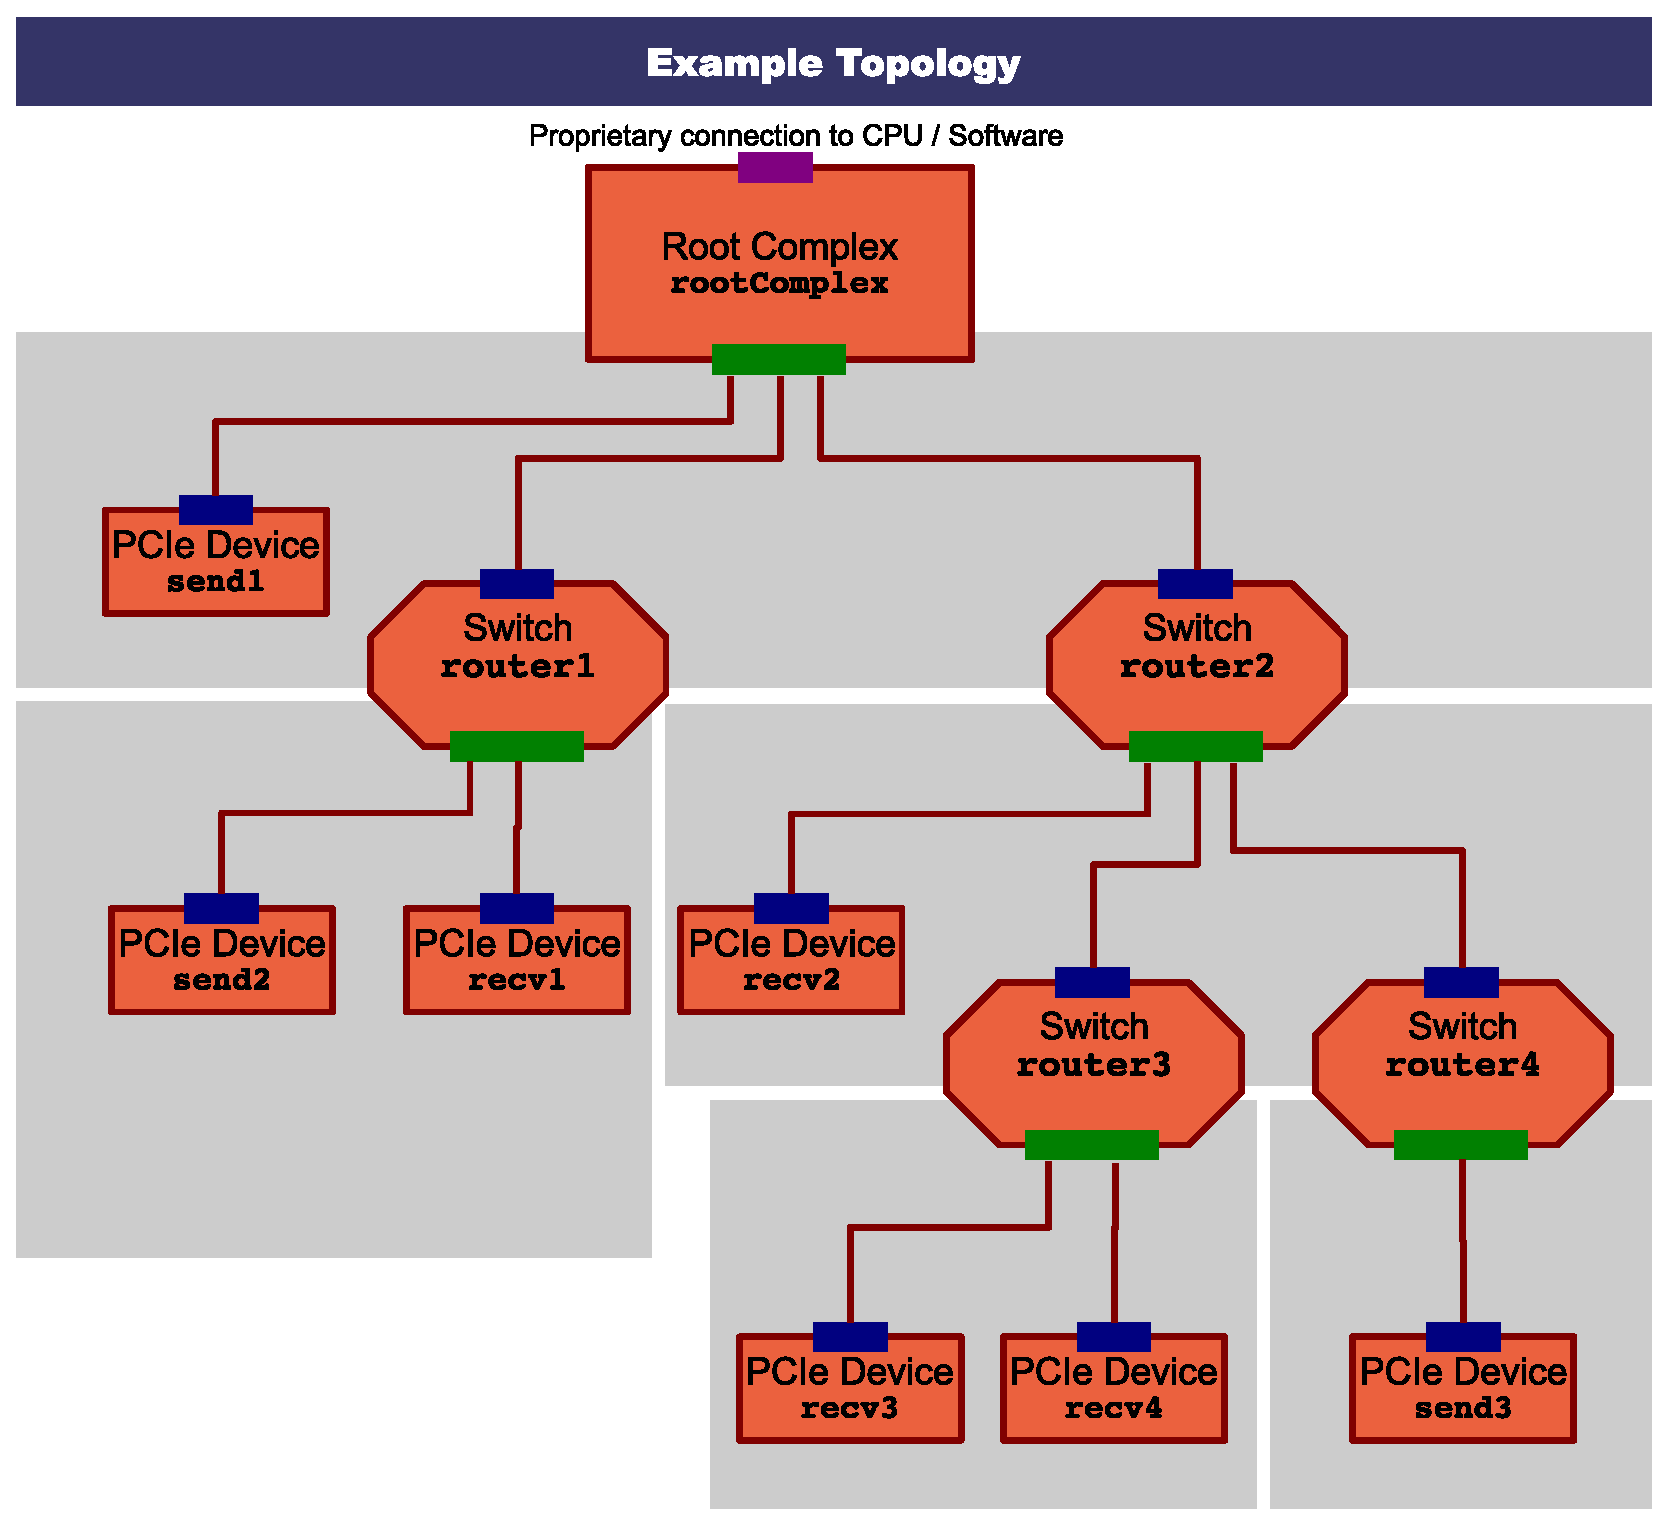
\includegraphics[width=15cm]{figures/example_pcie_platform_topology.eps}} 
	\caption{Example topology.}
	\label{fig:ExampleTopology}
\end{figure}

\begin{figure}[htbp]
  \begin{lstlisting}
#include "my_globals.h"
#include "greenbus/transport/PCIe/PCIe.h"
#include "greenbus/transport/PCIe/PCIeRouter.h"
#include "MyPCIeRootComplex.h"
#include "PCIeSendDevice.h"
#include "PCIeRecvDevice.h"
                              
int sc_main(int, char**)
{
  // instantiate partizipants
  MyPCIeRootComplex rootComplex("rootComplex");
  PCIeRecvInfoDevice recv1("recv1");
  PCIeRecvInfoDevice recv2("recv2");
  PCIeRecvInfoDevice recv3("recv3");
  PCIeRecvInfoDevice recv4("recv4");
  PCIeSendDevice     send1("send1");
  PCIeSendDevice     send2("send2");
  PCIeSendDevice     send3("send3");
  PCIeRouter router1("router1");
  PCIeRouter router2("router2");
  PCIeRouter router3("router3");
  PCIeRouter router4("router4");

  // connect Devices
  rootComplex.downstream_port(send1.mAPI);

  router1.upstream_port(rootComplex.downstream_port);
  router1.downstream_port(send2.mAPI);
  router1.downstream_port(recv1.mAPI);

  router2.upstream_port(rootComplex.downstream_port);
  router2.downstream_port(recv2.mAPI);

  router3.upstream_port(router2.downstream_port);
  router3.downstream_port(recv3.mAPI);
  router3.downstream_port(recv4.mAPI);

  router4.upstream_port(router2.downstream_port);
  router4.downstream_port(send3.mAPI);

  // start simulation
  sc_start();
  return 0;
} 
  \end{lstlisting}
  \caption{Example top-level testbench.}
  \label{fig:lstExampleTopology}
\end{figure}

%%%%%%%%%%%%%%%%%%%%%%%%%%%%%%%%%%%%%%%%%%%
\section{Mix Generic and PCIe Devices}
\label{sec:MixGenericAndPCIeDevices}

This section describes how a generic device can be connected to a PCIe topology using the extension mechanism.

%%%%%
\subsection{How to connect Generic Devices to PCIe Switches?}
\label{sec:HowConnGenDev2PCIeRouter}

The main precondition for getting generic devices compatible to be connected to a PCIe topology is that the generic device has to use PCIe Transactions and ports.

%%%
\subsubsection{Introduction}
In a generic device the included header is \Datei{GP.h} (see section \ref{sec:IncludePCIe}). This include has to typedef PCIe Transactions (and other classes) to generic ones. This is done either by changing the include to \Datei{greenbus/transport/PCIe/PCIe.h} or by using the make switch (see section \ref{sec:IncludePCIe}). Afterwards PCIe transactions are created instead of generic transactions while keeping the same generic API. 

Generic transactions are address based so the compatibility API creates PCIe MemoryRead/Write transactions in parallel to generic transactions. 

\Note{Implementation Note}{Generic Devices in a PCIe topology}{For this behavior, the convenience access methods in the PCIe Access classes which are used by the generic device have to be adapted. E.g. \lstinline|setMCmd(..)| sets the PCIe quark \lstinline|MPCIeCmd| instead of (more precisely in addition to) \lstinline|MCmd|.}

Now the generic devices can be connected to the PCIe port of the router. If the generic device has two ports (initiator\_port and target\_port) it has to be connected to the router twice. This is no issue for configuration because generic devices don't understand any ID routed TLPs anyway.

Generic Read and Write Transactions have an equivalent in PCIe: Memory Read and Write Transactions. Due to this analogy it is possible to map generic Generic\_MCMD\_RD and Generic\_MCMD\_WR transactions to PCIe MemRead and MemWrite transactions.

\Note{Implementation Note}{Mapping Generic Command Type to PCIe Command type}{PCIe uses an own Command enumeration because the generic one is not extendable. The two analogical transactions have the same number.}

The supported features are: Read, Write Transactions, Error handling, Completion / BytesValid.

%%%
\subsubsection{User View}
To connect modules which use generic ports (\lstinline|initiator_port|, \lstinline|target_port|,...) to PCIe modules or routers the user has to do the following steps (see example \Verzeichnis{examples/PCIe/generic/}):
\begin{itemize}
  \item Make sure to use the PCIe typedefs for generic classes in the generic modules (either include \DateiNoImg{PCIe.h} or use make switch).
  \item Instantiate the modules and routers as usual in the testbench.
  \item Manually set the address range of the generic module:
    \begin{lstlisting}
gen_s.target_port.base_addr = (MAddr) 0x0000000000000000LL;
gen_s.target_port.high_addr = (MAddr) 0x000000000000FFFFLL;
    \end{lstlisting}
  \item Connect the generic device to a PCIe Router Downstream Port like it is done with PCIe modules, e.g. 
    \begin{lstlisting}
router.downstream_port(gen_m.init_port);
router.downstream_port(gen_s.target_port);
    \end{lstlisting}
  \item Generate ID map after ''all'' connections are done:
    \begin{lstlisting}
router.m_PCIeAddressMap.generate_ID_map();
    \end{lstlisting}
  \item Manually register the generic address range at the router:
    \begin{lstlisting}
router.add_address_range(gen_s.target_port);
    \end{lstlisting}
\end{itemize}

%%%
\subsubsection{Alternative Connection}
An alternative to the direct connection is the \lstinline|PCIe2GenericPortWrapper| which was developed for connecting a PCIe Device to a Generic Router (see section \ref{sec:HowConnPCIe2GenRouters}). The wrapper maps the two ports of a master and slave Generic Device to one bidirectional PCIe port. 

Figure \ref{fig:ConnGenDev2PCIeSwitch} shows the available alternatives connecting a Generic Device to a PCIe Router.

\begin{figure}[H]%[htbp]
	\centerline{
		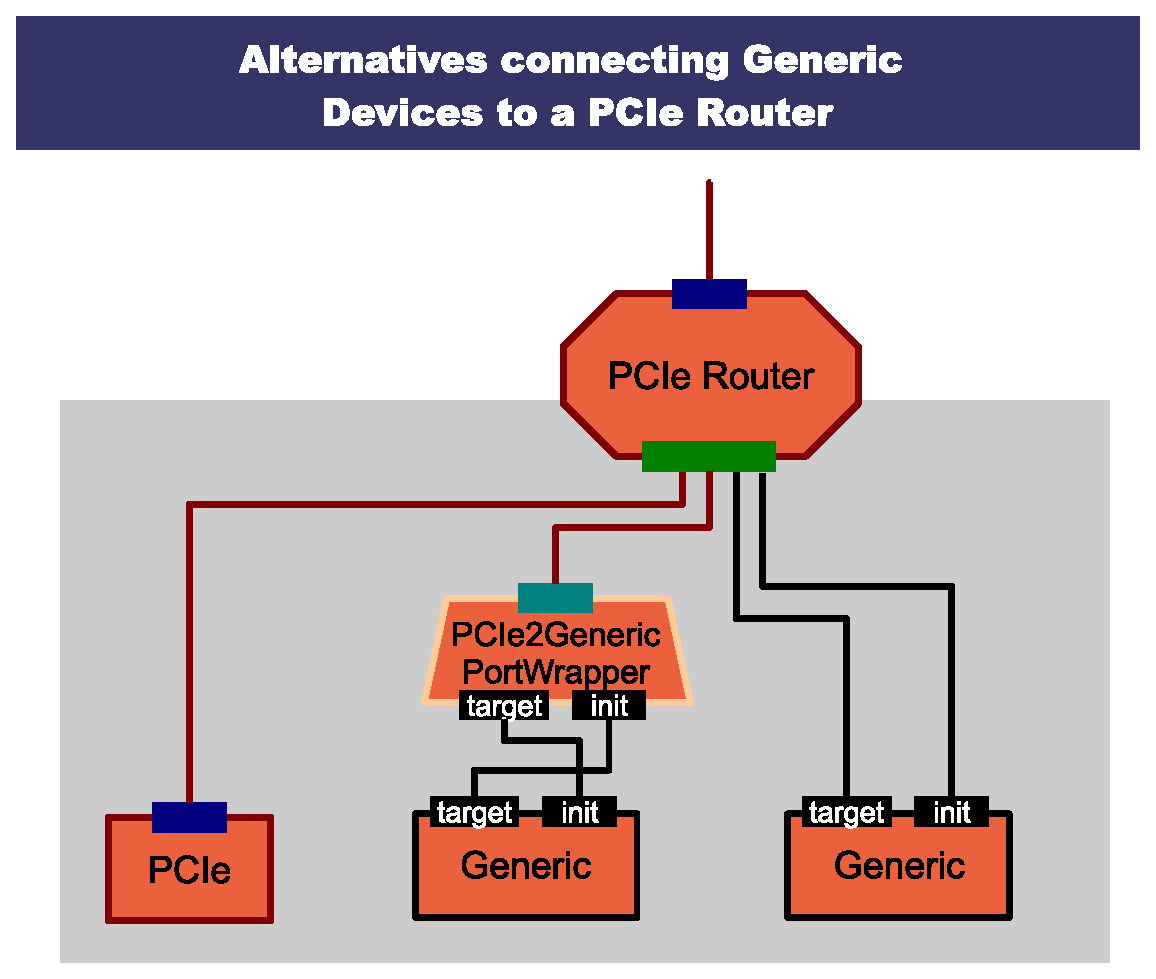
\includegraphics[width=13cm]{figures/Conn_GenericDev_PCIeRouter.eps} 
	}
	\caption{Alternative connections Generic Device to PCIe Switch}
	\label{fig:ConnGenDev2PCIeSwitch}
\end{figure}

%%%%%
\subsection{How to connect PCIe Devices to Generic Routers?}
\label{sec:HowConnPCIe2GenRouters}

A PCIe Device can be connected to a generic topology (e.g. router) if the generic modules use PCIe classes instead of generic ones (same precondition as in section \ref{sec:HowConnGenDev2PCIeRouter}). The PCIe Device only may send Memory Read and Memory Write TLPs. At the PCIe Device received generic reads and writes are mapped to PCIe Memory Reads and Memory Writes.

If the PCIe device is only a master or a slave (only sends or receives TLPs) the device may be connected directly to the \lstinline|init_port| or \lstinline|target_port| of the Generic Router. The user has to set the \lstinline|base_addr| and \lstinline|high_addr| parameters of the API port manually.

If the PCIe device should act as master \emph{and} slave a wrapper (\lstinline|PCIe2GenericPortWrapper|) has to be used to map the bidirectional PCIe port to an \lstinline|init_port| and a \lstinline|target_port|. Now the \lstinline|target_port| of the wrapper automatically gets the address range of the PCIe port (during before\_end\_of\_elaboration).

This wrapper class in in \Datei{greenbus/protocol/PCIe/PCIeGenericWrapper.h}. The listing in figure \ref {fig:lstWrapper} shows how to use this wrapper. 

\begin{figure}[H]%[htbp]
	\begin{lstlisting}
#include "greenbus/protocol/PCIe/PCIeGenericWrapper.h"

// ... see greenbus/examples/PCIe/generic/

tlm::PCIe::PCIe2GenericPortWrapper wrapper_pcie_m("PCIe2GenericPortWrapper_pcie_m");
PCIeSendDevice3 pcie_m("PCIe_Master");

// Set Device's address range
pcie_m.mAPI.base_addr = (MAddr) 0x0000000000100000LL;
pcie_m.mAPI.high_addr = (MAddr) 0x00000000001FFFFFLL;

// Connect PCIe Device with wrapper (as Master and Slave)
r.init_port(wrapper_pcie_m.target_port);
wrapper_pcie_m.init_port(r.target_port);
wrapper_pcie_m.pcie_port(pcie_m.mAPI);
	\end{lstlisting}
	\caption{Connect PCIe Device to Generic Router with Wrapper.}
	\label{fig:lstWrapper}
\end{figure}

An example using this wrapper (and comments for not using the wrapper) is in the example \Verzeichnis{greenbus/examples/PCIe/generic/} (define \lstinline|USE_GENERIC_ROUTER_CONNECT|).

Figure \ref{fig:ConnPCIeDev2GenRouter} shows the available alternatives connecting a PCIe Device to a Generic Router.

\begin{figure}[H]%[htbp]
	\centerline{
		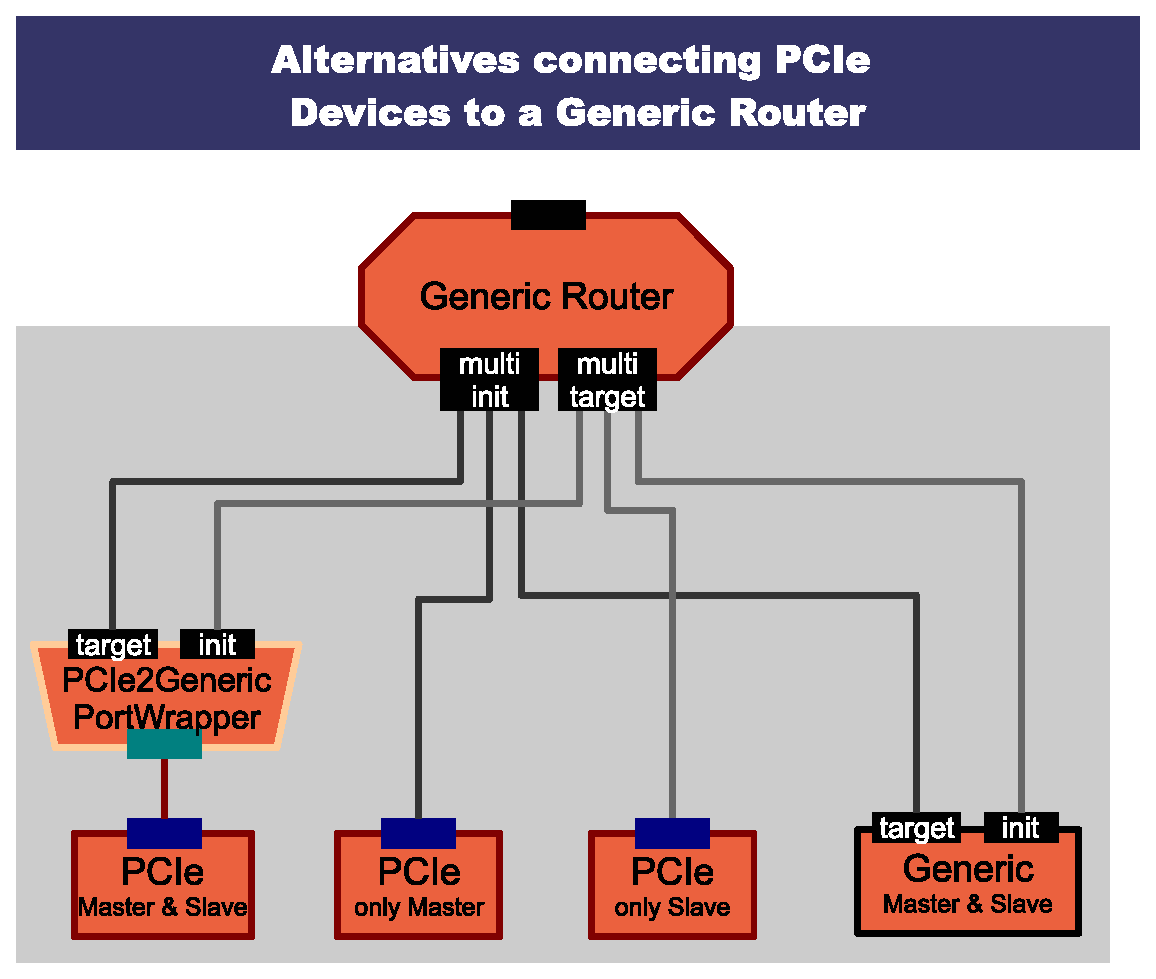
\includegraphics[width=13cm]{figures/Conn_PCIeDev_GenericRouter.eps} 
	}
	\caption{Alternative connections PCIe Device to Generic Router}
	\label{fig:ConnPCIeDev2GenRouter}
\end{figure}


%%%%%%%%%%%%%%%%%%%%%%%%%%%%%%%%%%%%%%%%%%%
\section{Specials}
\label{sec:Specials}

This sections is a collection of some special TLPs etc.

%%%%%
\subsection{Interrupts}
Legacy support interrupts are provided by with INTx Messages (Assert/Deassert) which can be generated with the transaction access methods. The PCIe Router has to handle these Interrupt messages in a special way.

The PCIe Router supports a basic mechanism handling INTx Assert and Deassert Messages: An (Downstream) incoming Interrupt Message is terminated at the receiver (Switch) (see MessageType). The Interrupt is forwarded after calculating the mapping. This approach does not match all requirements (see Specification pages 72f.) but will care for forwarding the correct Message. (Not supported e.g.: Interrupt Disable bit of the Command register, Deassert Message in the case of DL\_Down, Root Complex support.)

%%%%%
\subsection{Power Management Turn Off Message and Ack}
The acknowledgment to the Power Management message PME\_Turn\_Off is a special routing case: The Turn\_Off message is broadcasted to all devices and each device has to react with a PME\_TO\_Ack message. A Switch has to forward the Ack only after having received all Acks from its downstream devices. A Switch counts the incoming PME\_TO\_Ack messages and sends the PME\_TO\_Ack message to its upstream port after having received Acks from all Downstream Ports.
